\documentclass{article}
\usepackage[a4paper, margin=0.5in]{geometry}
\usepackage{tikz}
\usepackage{listings}
\usepackage[dvipsnames]{xcolor}
\usepackage{amsmath, amssymb, mathtools}
\usepackage{hyperref}
\usepackage{pgfplots}
\usepackage{graphicx}
\usetikzlibrary{calc}
\usetikzlibrary{intersections}
\usetikzlibrary{decorations.fractals,spy}
\usetikzlibrary{arrows.meta}
\usetikzlibrary{arrows}
\usetikzlibrary{shapes.geometric, shapes.symbols}
\usetikzlibrary{positioning}

\pgfplotsset{compat=newest}

\lstset{
  language=[LaTeX]TeX,
  basicstyle=\ttfamily\small,       % font style/size
  keywordstyle=\color{blue},        % keywords
  commentstyle=\color{Green},        % comments
  stringstyle=\color{red},          % strings
  backgroundcolor=\color{black!5},  % light gray background
  frame=single,                     % box around code
  rulecolor=\color{black!50},       % frame color
  numbers=left,                     % line numbers on the left
  numberstyle=\tiny\color{gray},    % line number style
  stepnumber=1,                     % number every line
  numbersep=8pt,                    % distance code ↔ numbers
  showstringspaces=false,           % don’t mark spaces in strings
  tabsize=2,                        % tab size
  breaklines=true,                  % wrap long lines
  breakatwhitespace=true,           % wrap only at whitespace
  captionpos=b                      % captions at the bottom
}

\title{\textbf{TikZ Tutorial}}
\author{\href{mailto:marcel.sayegh@rwth-aachen.de}{\texttt{marcel.sayegh@rwth-aachen.de}}}
\date{}

\begin{document}
\maketitle

\section{TikZ Evvironment in \LaTeX}

\subsubsection*{General Setup}
\begin{minipage}[c]{0.49\textwidth}
\begin{lstlisting}
\documentclass{...}
\usepackage{tikz}

\begin{document}

\begin{tikzpicture}
  % TikZ commands for cool visualization
\end{tikzpicture}

\end{document}
\end{lstlisting}
\end{minipage}
\hfill
\begin{minipage}[c]{0.49\textwidth}
  \centering

  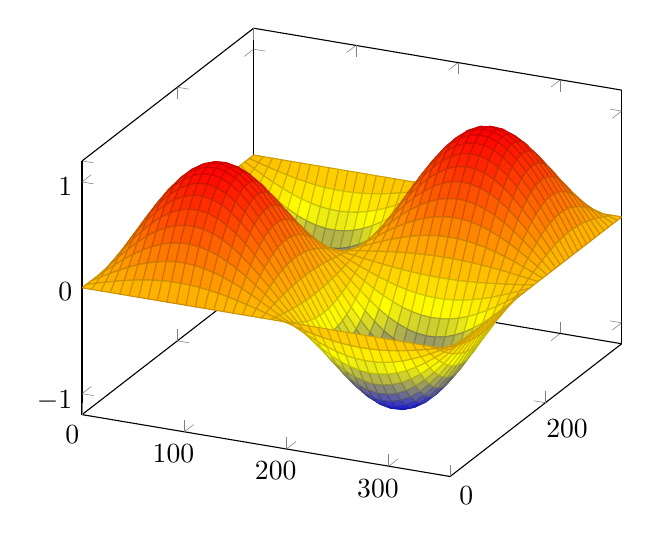
\begin{tikzpicture}
    \begin{axis}
      \addplot3[surf,domain=0:360,samples=40]
      {sin(x)*sin(y)};
    \end{axis}
  \end{tikzpicture}
\end{minipage}


\section{Relative and calculated coordinates}

\subsubsection*{Relative Coordinates (Vector Addition)}
\begin{minipage}[c]{0.7\textwidth}
\begin{lstlisting}
\begin{tikzpicture}
  ...
  % ++ Remembers last coordinate
  \draw (0,0) -- ++(2,0) -- ++(0,2) -- ++(2,0) -- ++(0,2);
  ...
\end{tikzpicture}
\end{lstlisting}
\end{minipage}
\hfill
\begin{minipage}[c]{0.29\textwidth}
  \centering
  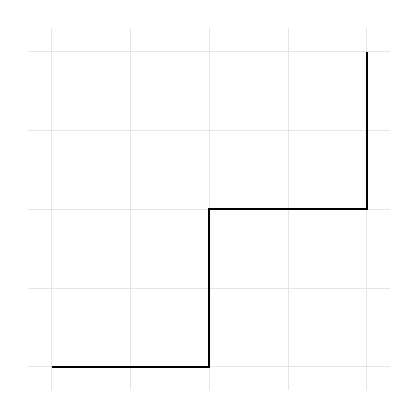
\begin{tikzpicture}
    \draw[gray!20] (-0.3,-0.3) grid (4.3,4.3);
    \draw[thick] (0,0) -- ++(2,0) -- ++(0,2) -- ++(2,0) -- ++(0,2);
  \end{tikzpicture}
\end{minipage}
\begin{minipage}[c]{0.7\textwidth}
\begin{lstlisting}
\begin{tikzpicture}
  ...
  % + Remembers only first coordinate
  \draw (0,0) -- +(2,0) -- +(0,2);
  ...
\end{tikzpicture}
\end{lstlisting}
\end{minipage}
\hfill
\begin{minipage}[c]{0.29\textwidth}
  \centering
  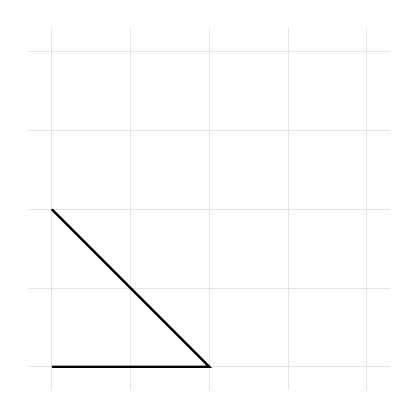
\begin{tikzpicture}
    \draw[gray!20] (-0.3,-0.3) grid (4.3,4.3);
    \draw[thick] (0,0) -- +(2,0) -- +(0,2);
  \end{tikzpicture}
\end{minipage}

\subsubsection*{Defining Coordinates}
\begin{minipage}[c]{0.7\textwidth}
\begin{lstlisting}
\begin{tikzpicture}
  ...
  \coordinate (A) at (0,0);
  \coordinate (B) at (0,2);

  \fill[red] (A) circle (2pt);
  \fill[blue] (B) circle (2pt);

  % Shorthand
  % \fill[red]  (A) at (0,0) circle (2pt);
  % \fill[blue] (B) at (0,2) circle (2pt);
  ...
\end{tikzpicture}
\end{lstlisting}
\end{minipage}
\hfill
\begin{minipage}[c]{0.29\textwidth}
  \centering
  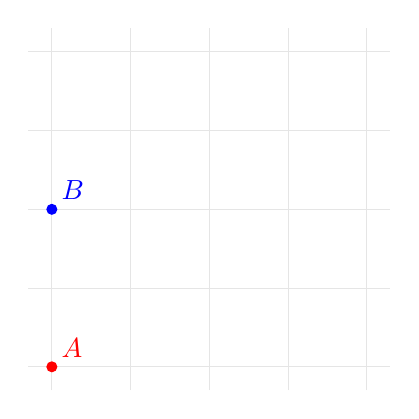
\begin{tikzpicture}
    \draw[gray!20] (-0.3,-0.3) grid (4.3,4.3);
    \coordinate (A) at (0,0);
    \coordinate (B) at (0,2);

    \fill[red] (A) circle (2pt) node[above right] {$A$};
    \fill[blue] (B) circle (2pt) node[above right] {$B$};
  \end{tikzpicture}
\end{minipage}

\subsubsection*{Arithmetic with coordinates}
\begin{minipage}[c]{0.7\textwidth}
\begin{lstlisting}
\usetikzlibrary{calc} % Import necessary

\begin{tikzpicture}
  ...
  \coordinate (A) at (0,0);
  \coordinate (B) at (0,2);
  \coordinate (C) at ($(A) + 2*(B)$);

  \fill[red] (A) circle (2pt);
  \fill[blue] (B) circle (2pt);
  \fill[Green] (C) circle (2pt);
  ...
\end{tikzpicture}
\end{lstlisting}
\end{minipage}
\hfill
\begin{minipage}[c]{0.29\textwidth}
  \centering
  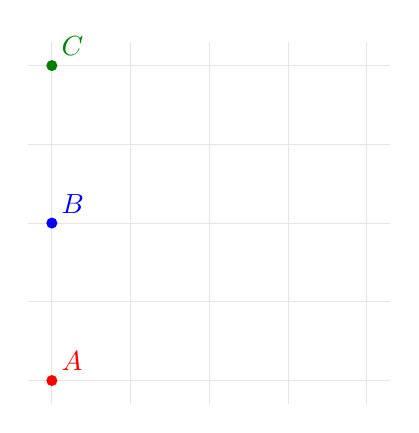
\begin{tikzpicture}
    \draw[gray!20] (-0.3,-0.3) grid (4.3,4.3);
    \coordinate (A) at (0,0);
    \coordinate (B) at (0,2);
    \coordinate (C) at ($(A) + 2*(B)$);

    \fill[red] (A) circle (2pt) node[above right] {$A$};
    \fill[blue] (B) circle (2pt) node[above right] {$B$};
    \fill[Green] (C) circle (2pt) node[above right] {$C$};
  \end{tikzpicture}
\end{minipage}

\subsubsection*{Projected Points}
\begin{minipage}[c]{0.7\textwidth}
\begin{lstlisting}
\begin{tikzpicture}
  ...
  \coordinate (A) at (0,0);
  \coordinate (B) at (3,4);
  \coordinate (C) at (0.5,2.5);

  \fill[red] (A) circle (2pt);
  \fill[blue] (B) circle (2pt);
  \fill[green] (C) circle (2pt);
  \fill[purple] ($(A)!(C)!(B)$) circle (2pt);
  ...
\end{tikzpicture}
\end{lstlisting}
\end{minipage}
\hfill
\begin{minipage}[c]{0.29\textwidth}
  \centering
  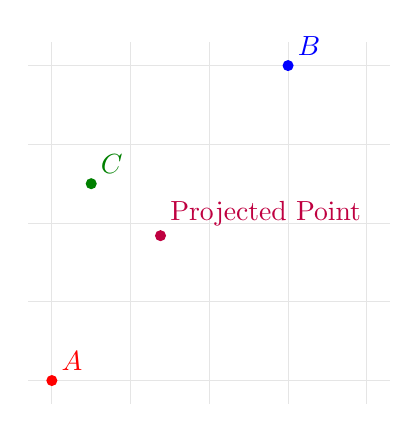
\begin{tikzpicture}
    \draw[gray!20] (-0.3,-0.3) grid (4.3,4.3);
    \coordinate (A) at (0,0);
    \coordinate (B) at (3,4);
    \coordinate (C) at (0.5,2.5);

    \fill[red] (A) circle (2pt) node[above right] {$A$};
    \fill[blue] (B) circle (2pt) node[above right] {$B$};
    \fill[Green] (C) circle (2pt) node[above right] {$C$};
    \fill[purple] ($(A)!(C)!(B)$) circle (2pt) node[above right] {Projected Point};
  \end{tikzpicture}
\end{minipage}

\subsubsection*{Intersections}
\begin{minipage}[c]{0.7\textwidth}
\begin{lstlisting}
\usetikzlibrary{intersections} % Import necessary

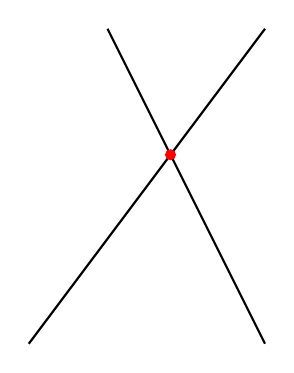
\begin{tikzpicture}
  ...
  \draw[name path=vector1, thick] (0,0) -- (3,4);
  \draw[name path=vector2, thick] (3,0) -- (1,4);
  \fill[name intersections={of=vector1 and vector2, by=intersectionPoint}, red] (intersectionPoint) circle (2pt);
  ...
\end{tikzpicture}
\end{lstlisting}
\end{minipage}
\hfill
\begin{minipage}[c]{0.29\textwidth}
  \centering
  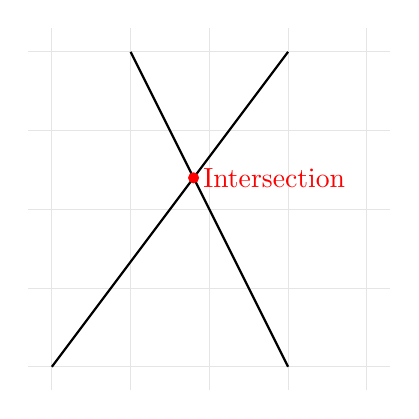
\begin{tikzpicture}
    \draw[gray!20] (-0.3,-0.3) grid (4.3,4.3);
    \draw[name path=vector1, thick] (0,0) -- (3,4);
    \draw[name path=vector2, thick] (3,0) -- (1,4);
    \fill[name intersections={of=vector1 and vector2, by=intersectionPoint}, red] (intersectionPoint) circle (2pt) node[right] {Intersection};
  \end{tikzpicture}
\end{minipage}

\subsubsection*{Paths}

\begin{minipage}[c]{0.7\textwidth}
\begin{lstlisting}
\usetikzlibrary{intersections} % Import necessary

\begin{tikzpicture}
  ...
  % Not drawn but still exists
  \path[name path=vector1, thick] (0,0) -- (3,4);
  \draw[name path=vector2, thick] (3,0) -- (1,4);
  \fill[name intersections={of=vector1 and vector2, by=intersectionPoint}, red] (intersectionPoint) circle (2pt);
  ...
\end{tikzpicture}
\end{lstlisting}
\end{minipage}
\hfill
\begin{minipage}[c]{0.29\textwidth}
  \centering
  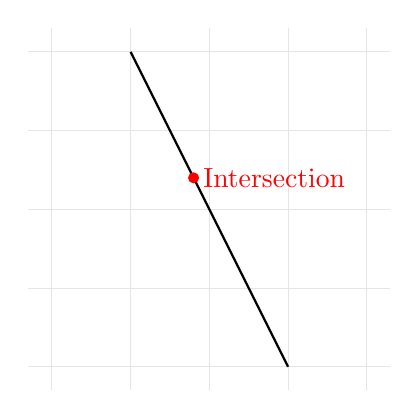
\begin{tikzpicture}
    \draw[gray!20] (-0.3,-0.3) grid (4.3,4.3);
    \path[name path=vector1, thick] (0,0) -- (3,4);
    \draw[name path=vector2, thick] (3,0) -- (1,4);
    \fill[name intersections={of=vector1 and vector2, by=intersectionPoint}, red] (intersectionPoint) circle (2pt) node[right] {Intersection};
  \end{tikzpicture}
\end{minipage}

\section{Options and Keys}

\subsubsection*{Common Options (Line thickness)}

\begin{minipage}[c]{0.7\textwidth}
\begin{lstlisting}

\begin{tikzpicture}
  ...
  \draw                   (0,0) -- (4,0);         % 0.4pt
  \draw[ultra thin]       (0.0,0.5) -- (4.0,0.5); % 0.1pt
  \draw[very thin]        (0.0,1.0) -- (4.0,1.0); % 0.2pt
  \draw[thin]             (0.0,1.5) -- (4.0,1.5); % 0.4pt
  \draw[semithick]        (0.0,2.0) -- (4.0,2.0); % 0.6pt
  \draw[thick]            (0.0,2.5) -- (4.0,2.5); % 0.8pt
  \draw[very thick]       (0.0,3.0) -- (4.0,3.0); % 1.2pt
  \draw[ultra thick]      (0.0,3.5) -- (4.0,3.5); % 1.6pt
  \draw[line width=4.2pt] (0.0,4.0) -- (4.0,4.0); % 4.2pt
  ...
\end{tikzpicture}
\end{lstlisting}
\end{minipage}
\hfill
\begin{minipage}[c]{0.29\textwidth}
  \centering
  
\begin{tikzpicture}
    \draw[gray!20] (-0.3,-0.3) grid (4.3,4.3);
    \draw (0,0) -- (4,0);
    \draw[ultra thin] (0.0,0.5) -- (4.0,0.5);
    \draw[very thin] (0.0,1.0) -- (4.0,1.0);
    \draw[thin] (0.0,1.5) -- (4.0,1.5);
    \draw[semithick] (0.0,2.0) -- (4.0,2.0);
    \draw[thick] (0.0,2.5) -- (4.0,2.5);
    \draw[very thick] (0.0,3.0) -- (4.0,3.0);
    \draw[ultra thick] (0.0,3.5) -- (4.0,3.5);
    \draw[line width=4.2pt] (0.0,4.0) -- (4.0,4.0);
  \end{tikzpicture}
\end{minipage}
\subsubsection*{Common Options (Dash Patterns)}
\begin{minipage}[c]{0.7\textwidth}
\begin{lstlisting}
\begin{tikzpicture}
  ...
  % Dash Patterns
  \draw                       (0,0.0) -- (4,0.0);
  \draw[solid]                (0,0.3) -- (4,0.3);
  \draw[dashed]               (0,0.6) -- (4,0.6);
  \draw[densely dashed]       (0,0.9) -- (4,0.9);
  \draw[loosely dashed]       (0,1.2) -- (4,1.2);
  \draw[dotted]               (0,1.5) -- (4,1.5);
  \draw[densely dotted]       (0,1.8) -- (4,1.8);
  \draw[loosely dotted]       (0,2.1) -- (4,2.1);
  \draw[dash dot]             (0,2.4) -- (4,2.4);
  \draw[densely dash dot]     (0,2.7) -- (4,2.7);
  \draw[loosely dash dot]     (0,3.0) -- (4,3.0);
  \draw[dash dot dot]         (0,3.3) -- (4,3.3);
  \draw[densely dash dot dot] (0,3.6) -- (4,3.6);
  \draw[loosely dash dot dot] (0,3.9) -- (4,3.9);
  ...
\end{tikzpicture}
\end{lstlisting}
\end{minipage}
\hfill
\begin{minipage}[c]{0.29\textwidth}
  \centering
  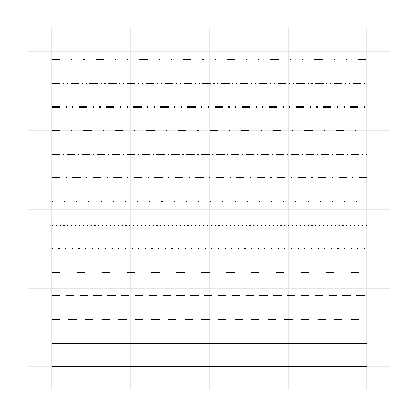
\begin{tikzpicture}
    \draw[gray!20] (-0.3,-0.3) grid (4.3,4.3);

    \draw (0,0.0) -- (4,0.0);
    \draw[solid] (0,0.3) -- (4,0.3);
    \draw[dashed] (0,0.6) -- (4,0.6);
    \draw[densely dashed] (0,0.9) -- (4,0.9);
    \draw[loosely dashed] (0,1.2) -- (4,1.2);
    \draw[dotted] (0,1.5) -- (4,1.5);
    \draw[densely dotted] (0,1.8) -- (4,1.8);
    \draw[loosely dotted] (0,2.1) -- (4,2.1);
    \draw[dash dot] (0,2.4) -- (4,2.4);
    \draw[densely dash dot] (0,2.7) -- (4,2.7);
    \draw[loosely dash dot] (0,3.0) -- (4,3.0);
    \draw[dash dot dot] (0,3.3) -- (4,3.3);
    \draw[densely dash dot dot] (0,3.6) -- (4,3.6);
    \draw[loosely dash dot dot] (0,3.9) -- (4,3.9);
  \end{tikzpicture}
\end{minipage}
\subsubsection*{Common Options (Colors and Opacity)}
\begin{minipage}[c]{0.7\textwidth}
\begin{lstlisting}
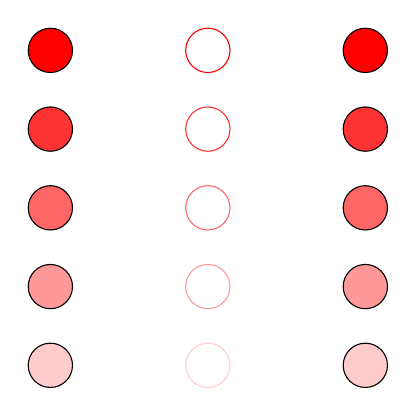
\begin{tikzpicture}
  ...
  % Fill opacities
  \draw[fill=red, fill opacity=0.2]  (0,0) circle (8pt);
  \draw[fill=red, fill opacity=0.4]  (0,1) circle (8pt);
  \draw[fill=red, fill opacity=0.6]  (0,2) circle (8pt);
  \draw[fill=red, fill opacity=0.8]  (0,3) circle (8pt);
  \draw[fill=red, fill opacity=1]    (0,4) circle (8pt);

  % Stroke opacities
  \draw[draw=red, draw opacity=0.2]  (2,0) circle (8pt);
  \draw[draw=red, draw opacity=0.4]  (2,1) circle (8pt);
  \draw[draw=red, draw opacity=0.6]  (2,2) circle (8pt);
  \draw[draw=red, draw opacity=0.8]  (2,3) circle (8pt);
  \draw[draw=red, draw opacity=1]    (2,4) circle (8pt);

  % Reducing color intensity (color mixing with white)
  \draw[fill=red!20]                 (4,0) circle (8pt);
  \draw[fill=red!40]                 (4,1) circle (8pt);
  \draw[fill=red!60]                 (4,2) circle (8pt);
  \draw[fill=red!80]                 (4,3) circle (8pt);
  \draw[fill=red]                    (4,4) circle (8pt);
  ...
\end{tikzpicture}
\end{lstlisting}
\end{minipage}
\hfill
\begin{minipage}[c]{0.29\textwidth}
  \centering
  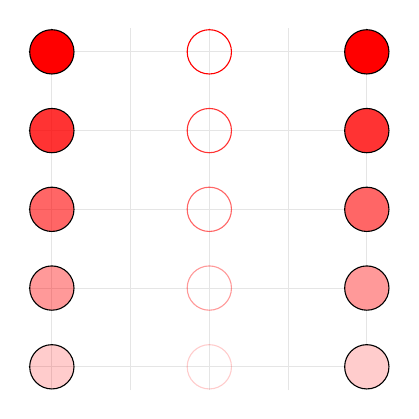
\begin{tikzpicture}
    \draw[gray!20] (-0.3,-0.3) grid (4.3,4.3);

    % Fill opacities
    \draw[fill=red, fill opacity=0.2]  (0,0) circle (8pt);
    \draw[fill=red, fill opacity=0.4]  (0,1) circle (8pt);
    \draw[fill=red, fill opacity=0.6]  (0,2) circle (8pt);
    \draw[fill=red, fill opacity=0.8]  (0,3) circle (8pt);
    \draw[fill=red, fill opacity=1]    (0,4) circle (8pt);

    % Stroke opacities
    \draw[draw=red, draw opacity=0.2]  (2,0) circle (8pt);
    \draw[draw=red, draw opacity=0.4]  (2,1) circle (8pt);
    \draw[draw=red, draw opacity=0.6]  (2,2) circle (8pt);
    \draw[draw=red, draw opacity=0.8]  (2,3) circle (8pt);
    \draw[draw=red, draw opacity=1]    (2,4) circle (8pt);

    % Reducing color intensity (color mixing with white)
    \draw[fill=red!20]  (4,0) circle (8pt);
    \draw[fill=red!40]  (4,1) circle (8pt);
    \draw[fill=red!60]  (4,2) circle (8pt);
    \draw[fill=red!80]  (4,3) circle (8pt);
    \draw[fill=red]     (4,4) circle (8pt);
  \end{tikzpicture}
\end{minipage}

\subsubsection*{Common Options (Line Caps)}

\begin{minipage}[c]{0.7\textwidth}
\begin{lstlisting}
\begin{tikzpicture}
  ...
  \draw[line cap=round] (0,0.5) -- (4,0.5);
  \draw[line cap=rect]  (0,2)   -- (4,2);
  \draw[line cap=butt]  (0,3.5) -- (4,3.5);
  ...
\end{tikzpicture}
\end{lstlisting}
\end{minipage}
\hfill
\begin{minipage}[c]{0.29\textwidth}
  \centering
  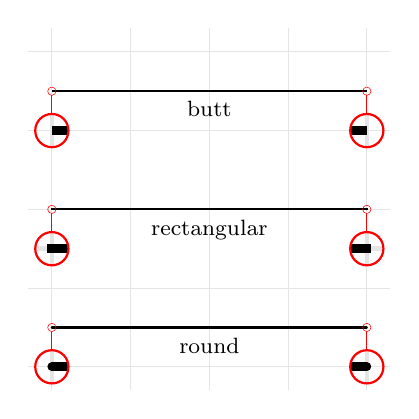
\begin{tikzpicture}[spy using outlines={circle, magnification=4, size=2cm, connect spies}]
    \draw[gray!20] (-0.3,-0.3) grid (4.3,4.3);
    % Caps
    \draw[line cap=round, thick]  (0,0.5) -- (4,0.5)
    node[midway, below, font=\footnotesize] {round};
    \spy[red, size=12pt] on (0,0.5) in node  at (0,0);
    \spy[red, size=12pt] on (4,0.5) in node  at (4,0);

    \draw[line cap=rect, thick]  (0,2) -- (4,2)
    node[midway, below, font=\footnotesize] {rectangular};
    \spy[red, size=12pt] on (0,2) in node  at (0,1.5);
    \spy[red, size=12pt] on (4,2) in node  at (4,1.5);

    \draw[line cap=butt, thick]  (0,3.5) -- (4,3.5)
    node[midway, below, font=\footnotesize] {butt};
    \spy[red, size=12pt] on (0,3.5) in node  at (0,3);
    \spy[red, size=12pt] on (4,3.5) in node  at (4,3);

  \end{tikzpicture}
\end{minipage}

\subsubsection*{Common Options (Line Joins)}

\begin{minipage}[c]{0.7\textwidth}
\begin{lstlisting}
\begin{tikzpicture}
  ...
  \draw[line join=miter]  (0,0)   -- (2,1)   -- (4,0);
  \draw[line join=round]  (0,1.5) -- (2,2.5) -- (4,1.5);
  \draw[line join=bevel]  (0,3)   -- (2,4)   -- (4,3);
  ...
\end{tikzpicture}
\end{lstlisting}
\end{minipage}
\hfill
\begin{minipage}[c]{0.29\textwidth}
  \centering
  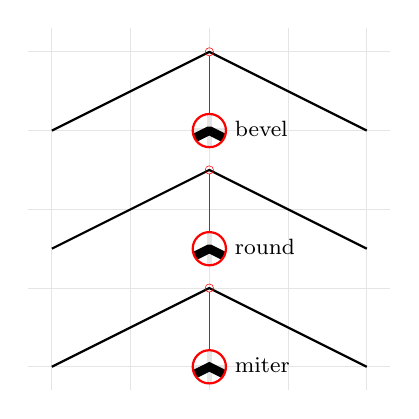
\begin{tikzpicture}[spy using outlines={circle, magnification=4, size=2cm, connect spies}]
    \draw[gray!20] (-0.3,-0.3) grid (4.3,4.3);
    % Joins
    \draw[line join=miter, thick]  (0,0) -- (2,1)  -- (4,0);
    \spy[red, size=12pt] on (2,1) in node  at (2,0);
    \node[right, font=\footnotesize] at (2.2,0.02) {miter};

    \draw[line join=round, thick]  (0,1.5) -- (2,2.5) -- (4,1.5);
    \spy[red, size=12pt] on (2,2.5) in node  at (2,1.5);
    \node[right, font=\footnotesize] at (2.2,1.52) {round};

    \draw[line join=bevel, thick]  (0,3) -- (2,4) -- (4,3);
    \spy[red, size=12pt] on (2,4) in node  at (2,3);
    \node[right, font=\footnotesize] at (2.2,3.02) {bevel};

  \end{tikzpicture}
\end{minipage}

\section{Nodes}
\subsubsection*{Node structure}
\begin{minipage}[c]{0.7\textwidth}
\begin{lstlisting}
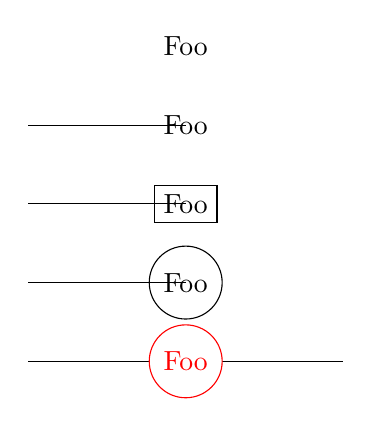
\begin{tikzpicture}
  ...
  % node[Optionen] (A) {};
  \draw (2,4) node {Foo};
  \draw (0,3) -- (2,3) node {Foo};
  \draw (0,2) -- (2,2) node[draw] {Foo};
  \draw (0,1) -- (2,1) node[draw, circle] {Foo};
  \draw (0,0) -- (2,0) node[draw, circle, red, fill=white] {Foo} -- (4,0);
  ...
\end{tikzpicture}
\end{lstlisting}
\end{minipage}
\hfill
\begin{minipage}[c]{0.29\textwidth}
  \centering
  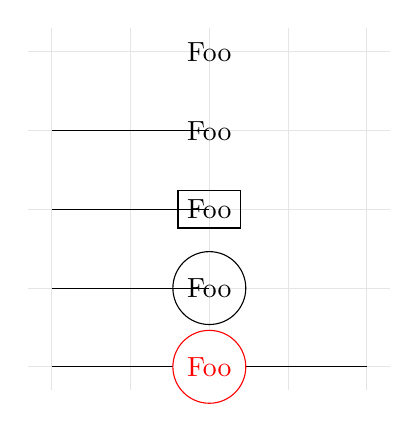
\begin{tikzpicture}[spy using outlines={circle, magnification=4, size=2cm, connect spies}]
    \draw[gray!20] (-0.3,-0.3) grid (4.3,4.3);

    \draw (2,4) node {Foo};
    \draw (0,3) -- (2,3) node {Foo};
    \draw (0,2) -- (2,2) node[draw] {Foo};
    \draw (0,1) -- (2,1) node[draw, circle] {Foo};
    \draw (0,0) -- (2,0) node[draw, circle, red, fill=white] {Foo} -- (4,0);

  \end{tikzpicture}
\end{minipage}

\subsubsection*{\textbackslash\texttt{node} operator}
\begin{minipage}[c]{0.7\textwidth}
\begin{lstlisting}
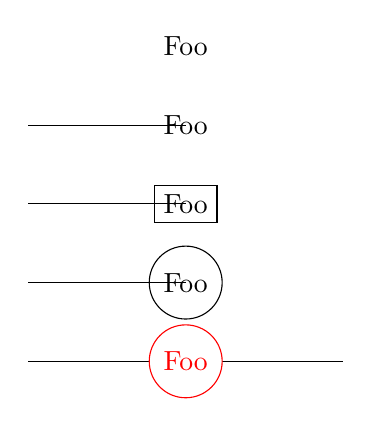
\begin{tikzpicture}
  ...
  % node[Optionen] (A) {};
  \draw (2,4) node {Foo};
  \draw (0,3) -- (2,3) node {Foo};
  \draw (0,2) -- (2,2) node[draw] {Foo};
  \draw (0,1) -- (2,1) node[draw, circle] {Foo};
  \draw (0,0) -- (2,0) node[draw, circle, red, fill=white] {Foo} -- (4,0);
  ...
\end{tikzpicture}
\end{lstlisting}
\end{minipage}
\hfill
\begin{minipage}[c]{0.29\textwidth}
  \centering
  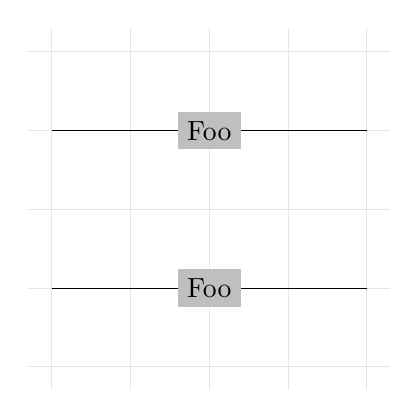
\begin{tikzpicture}[spy using outlines={circle, magnification=4, size=2cm, connect spies}]
    \draw[gray!20] (-0.3,-0.3) grid (4.3,4.3);
    % Instead of
    \draw (0,3) -- (2,3) node[fill=lightgray] {Foo} -- (4,3);

    % Can also do
    \draw (0,1) -- (4,1);
    \node[fill=lightgray] at (2,1) {Foo};

  \end{tikzpicture}
\end{minipage}

\subsubsection*{Common Node Shapes}

\begin{minipage}[c]{0.7\textwidth}
\begin{lstlisting}
\usetikzlibrary{shapes.geometric} % Import necessary
\usetikzlibrary{shapes.symbols}   % Import necessary

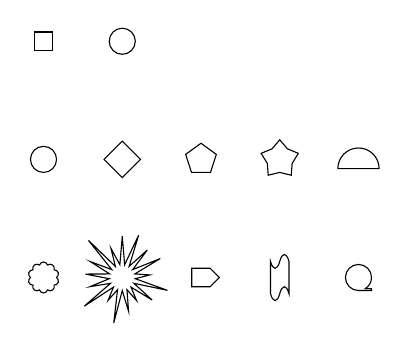
\begin{tikzpicture}
  ...
  % defaults shapes
  \node[draw, rectangle]       at (0,3) {};
  \node[draw, circle]          at  (1,3) {};

  % requires shapes.geometric
  \node[draw, ellipse]         at (0,1.5) {};
  \node[draw, diamond]         at (1,1.5) {};
  \node[draw, regular polygon] at (2,1.5) {};
  \node[draw, star]            at (3,1.5) {};
  \node[draw, semicircle]      at (4,1.5) {};

  % requires shapes.symbols
  \node[cloud, draw]           at (0,0) {};
  \node[starburst, draw]       at (1,0) {};
  \node[signal, draw]          at (2,0) {};
  \node[tape, draw]            at (3,0) {};
  \node[magnetic tape, draw]   at (4,0) {};
  ...
\end{tikzpicture}
\end{lstlisting}
\end{minipage}
\hfill
\begin{minipage}[c]{0.29\textwidth}
  \centering
  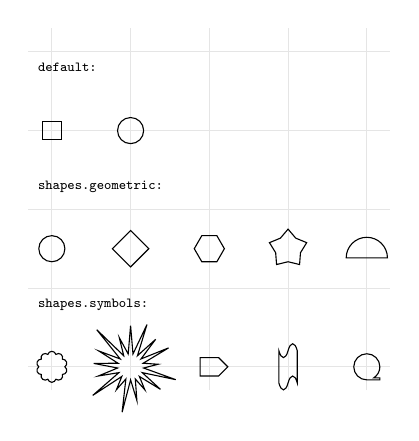
\begin{tikzpicture}[spy using outlines={circle, magnification=4, size=2cm, connect spies}]
    \draw[gray!20] (-0.3,-0.3) grid (4.3,4.3);
    \node[font=\tiny, anchor=base west] at (-0.3,3.75) {$\texttt{default:}$};
    \node[draw, rectangle] at (0,3) {};
    \node[draw, circle] at (1,3) {};

    \node[font=\tiny, anchor=base west] at (-0.3,2.25) {$\texttt{shapes.geometric:}$};
    \node[draw, ellipse] at (0,1.5) {};
    \node[draw, diamond] at (1,1.5) {};
    \node[draw, regular polygon, regular polygon sides=6] at (2,1.5) {};
    \node[draw, star]        at (3,1.5) {};
    \node[draw, semicircle]        at (4,1.5) {};

    \node[font=\tiny, anchor=base west] at (-0.3,0.75) {\texttt{shapes.symbols:}};
    \node[cloud, draw] at (0,0) {};
    \node[starburst, draw] at (1,0) {};
    \node[signal, draw] at (2,0) {};
    \node[tape, draw] at (3,0) {};
    \node[magnetic tape, draw] at (4,0) {};
  \end{tikzpicture}
\end{minipage}

\subsubsection*{Margin and padding}

\begin{minipage}[c]{0.7\textwidth}
\begin{lstlisting}
\begin{tikzpicture}
  ...
  \node[draw] (a) at (0,2) {A};
  \node[draw] (b) at (4,4) {B};
  \node[draw, inner sep=0] (c) at (4,2) {C}; % Padding
  \node[draw, outer sep=4] (d) at (4,0) {D}; % Margin

  \draw[->] (a) -- (b);
  \draw[->] (a) -- (c);
  \draw[->] (a) -- (d);
  ...
\end{tikzpicture}
\end{lstlisting}
\end{minipage}
\hfill
\begin{minipage}[c]{0.29\textwidth}
  \centering
  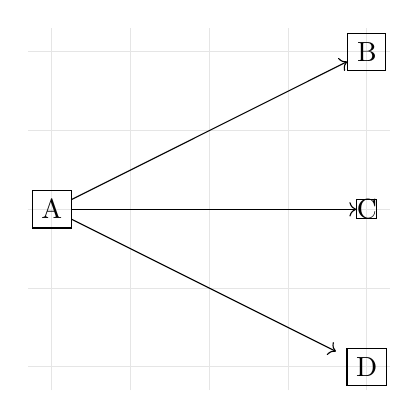
\begin{tikzpicture}[spy using outlines={circle, magnification=4, size=2cm, connect spies}]
    \draw[gray!20] (-0.3,-0.3) grid (4.3,4.3);

    \node[draw] (a) at (0,2) {A};
    \node[draw] (b) at (4,4) {B};
    \node[draw, inner sep=0] (c) at (4,2) {C}; % Padding
    \node[draw, outer sep=4] (d) at (4,0) {D}; % Margin

    \draw[->] (a) -- (b);
    \draw[->] (a) -- (c);
    \draw[->] (a) -- (d);
  \end{tikzpicture}
\end{minipage}

\subsubsection*{Positions}
\begin{minipage}[c]{0.7\textwidth}
\begin{lstlisting}
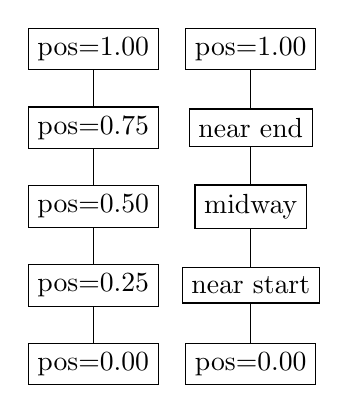
\begin{tikzpicture}
  ...
  \draw (1,0) -- (1,4)
  node[pos=0,       draw, fill=white]{pos=0.00}
  node[pos=0.25,    draw, fill=white]{pos=0.25}
  node[pos=0.5,     draw, fill=white]{pos=0.50}
  node[pos=0.75,    draw, fill=white]{pos=0.75}
  node[pos=1,       draw, fill=white]{pos=1.00}
  ;

  \draw (3,0) -- (3,4)
  node[pos=0,       draw, fill=white]{pos=0.00}
  node[near start,  draw, fill=white]{near start}
  node[midway,      draw, fill=white]{midway}
  node[near end,    draw, fill=white]{near end}
  node[pos=1,       draw, fill=white]{pos=1.00}
  ;
  ...
\end{tikzpicture}
\end{lstlisting}
\end{minipage}
\hfill
\begin{minipage}[c]{0.29\textwidth}
  \centering
  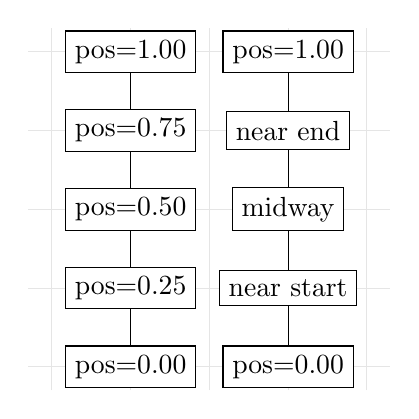
\begin{tikzpicture}[spy using outlines={circle, magnification=4, size=2cm, connect spies}]
    \draw[gray!20] (-0.3,-0.3) grid (4.3,4.3);
    \draw (1,0) -- (1,4)
    node[pos=0,     draw, fill=white]{pos=0.00}
    node[pos=0.25,  draw, fill=white]{pos=0.25}
    node[pos=0.5,   draw, fill=white]{pos=0.50}
    node[pos=0.75,  draw, fill=white]{pos=0.75}
    node[pos=1,     draw, fill=white]{pos=1.00}
    ;

    \draw (3,0) -- (3,4)
    node[pos=0,     draw, fill=white]{pos=0.00}
    node[near start,  draw, fill=white]{near start}
    node[midway,   draw, fill=white]{midway}
    node[near end,  draw, fill=white]{near end}
    node[pos=1,     draw, fill=white]{pos=1.00}
    ;
  \end{tikzpicture}
\end{minipage}

\subsubsection*{Sloping}
\begin{minipage}[c]{0.7\textwidth}
\begin{lstlisting}
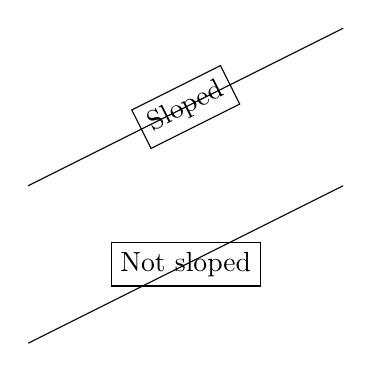
\begin{tikzpicture}
  ...
  \draw (0,0) -- (4,2) node[draw, midway] {Not sloped};
  \draw (0,2) -- (4,4) node[draw, midway, sloped] {Sloped};
  ...
\end{tikzpicture}
\end{lstlisting}
\end{minipage}
\hfill
\begin{minipage}[c]{0.29\textwidth}
  \centering
  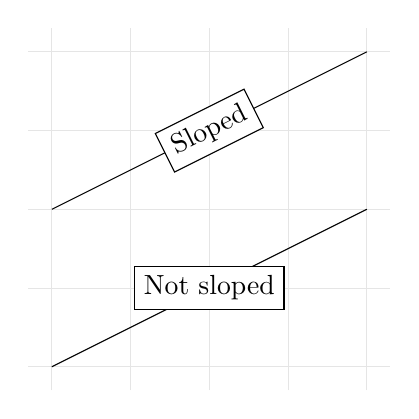
\begin{tikzpicture}[spy using outlines={circle, magnification=4, size=2cm, connect spies}]
    \draw[gray!20] (-0.3,-0.3) grid (4.3,4.3);
    \draw (0,0) -- (4,2) node[draw, fill=white, midway] {Not sloped};
    \draw (0,2) -- (4,4) node[draw, fill=white, midway, sloped] {Sloped};
  \end{tikzpicture}
\end{minipage}

\subsubsection*{Anchors}
\begin{minipage}[c]{0.7\textwidth}
\begin{lstlisting}
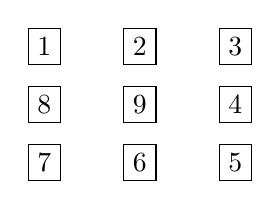
\begin{tikzpicture}
  ...
  \node[draw, above left]  at (1,4)   {1};
  \node[draw, above]       at (2,4)   {2};
  \node[draw, above right] at (3,4)   {3};
  \node[draw, right]       at (3,3.5) {4};
  \node[draw, below right] at (3,3)   {5};
  \node[draw, below]       at (2,3)   {6};
  \node[draw, below left]  at (1,3)   {7};
  \node[draw, left]        at (1,3.5) {8};
  \node[draw]              at (2,3.5) {9};
  ...
\end{tikzpicture}
\end{lstlisting}
\end{minipage}
\hfill
\begin{minipage}[c]{0.29\textwidth}
  \centering
  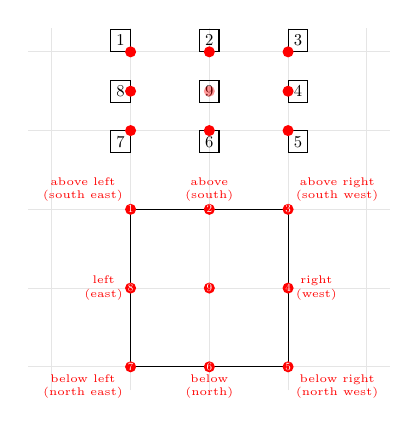
\begin{tikzpicture}[spy using outlines={circle, magnification=4, size=2cm, connect spies}]
    \draw[gray!20] (-0.3,-0.3) grid (4.3,4.3);

    \draw (1,0) -- (3,0) -- (3,2) -- (1,2) -- cycle;
    \fill[red] (1,0) circle (2pt) node[below left,  align=center, font=\tiny, scale=0.8]{below left\\(north east)};above left
    \fill[red] (2,0) circle (2pt) node[below,       align=center, font=\tiny, scale=0.8]{below\\(north)};above left
    \fill[red] (3,0) circle (2pt) node[below right, align=center, font=\tiny, scale=0.8]{below right\\(north west)};above left
    \fill[red] (3,1) circle (2pt) node[right,       align=center, font=\tiny, scale=0.8]{right\\(west)};above left
    \fill[red] (3,2) circle (2pt) node[above right, align=center, font=\tiny, scale=0.8]{above right\\(south west)};above left
    \fill[red] (2,2) circle (2pt) node[above,       align=center, font=\tiny, scale=0.8]{above\\(south)};above left
    \fill[red] (1,2) circle (2pt) node[above left,  align=center, font=\tiny, scale=0.8]{above left\\(south east)};above left
    \fill[red] (1,1) circle (2pt) node[left,        align=center, font=\tiny, scale=0.8]{left\\(east)};above left
    \fill[red] (2,1) circle (2pt);

    \node[text=white, scale=0.4] at (1,2) {1};
    \node[text=white, scale=0.4] at (2,2) {2};
    \node[text=white, scale=0.4] at (3,2) {3};
    \node[text=white, scale=0.4] at (3,1) {4};
    \node[text=white, scale=0.4] at (3,0) {5};
    \node[text=white, scale=0.4] at (2,0) {6};
    \node[text=white, scale=0.4] at (1,0) {7};
    \node[text=white, scale=0.4] at (1,1) {8};
    \node[text=white, scale=0.4] at (2,1) {9};

    \node[draw, above left, scale=0.6] at (1,4) {1};
    \fill[red] (1,4) circle (2pt);
    \node[draw, above, scale=0.6] at (2,4) {2};
    \fill[red] (2,4) circle (2pt);
    \node[draw, above right, scale=0.6] at (3,4) {3};
    \fill[red] (3,4) circle (2pt);
    \node[draw, right, scale=0.6] at (3,3.5) {4};
    \fill[red] (3,3.5) circle (2pt);
    \node[draw, below right, scale=0.6] at (3,3) {5};
    \fill[red] (3,3) circle (2pt);
    \node[draw, below, scale=0.6] at (2,3) {6};
    \fill[red] (2,3) circle (2pt);
    \node[draw, below left, scale=0.6] at (1,3) {7};
    \fill[red] (1,3) circle (2pt);
    \node[draw, left, scale=0.6] at (1,3.5) {8};
    \fill[red] (1,3.5) circle (2pt);
    \node[draw, anchor=center, scale=0.6] at (2,3.5) {9};
    \fill[red, opacity=0.4] (2,3.5) circle (2pt);

  \end{tikzpicture}
\end{minipage}

\section{\texttt{foreach} Loops}
\subsubsection*{Basic Looping}

\begin{minipage}[c]{0.7\textwidth}
\begin{lstlisting}
\begin{tikzpicture}
  ...
    \foreach \c in {0,1,2,3,4} {
      \draw (\c, 0) -- (\c, 2);
    }
  ...
\end{tikzpicture}
\end{lstlisting}
\end{minipage}
\hfill
\begin{minipage}[c]{0.29\textwidth}
  \centering
  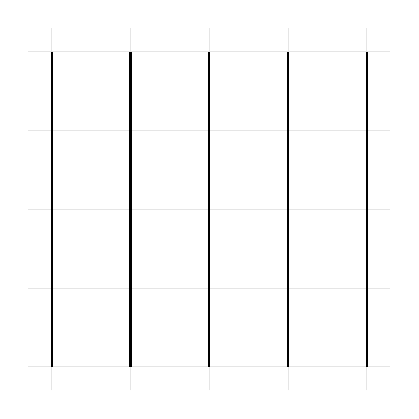
\begin{tikzpicture}
    \draw[gray!20] (-0.3,-0.3) grid (4.3,4.3);
    \foreach \c in {0,1,2,3,4} {
      \draw[thick] (\c, 0) -- (\c, 4);
    }
  \end{tikzpicture}
\end{minipage}

\subsubsection*{Automatic Ranges and Steps}

\begin{minipage}[c]{0.7\textwidth}
\begin{lstlisting}
\begin{tikzpicture}
  ...
  \foreach \angle in {0,20,...,340} {
    \fill ($(2,2) + (\angle:2)$) circle (2pt);
  }
  ...
\end{tikzpicture}
\end{lstlisting}
\end{minipage}
\hfill
\begin{minipage}[c]{0.29\textwidth}
  \centering
  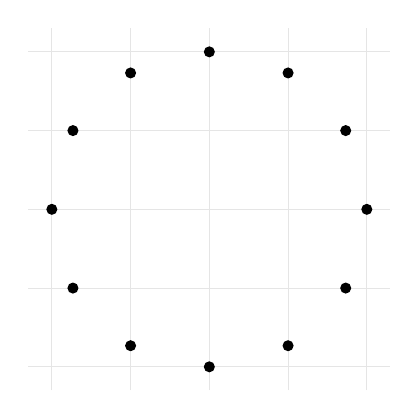
\begin{tikzpicture}
    \draw[gray!20] (-0.3,-0.3) grid (4.3,4.3);
    \foreach \angle in {0,30,...,330} {
      \fill ($(2,2) + (\angle:2)$) circle (2pt);
    }
  \end{tikzpicture}
\end{minipage}

\subsubsection*{Loop Indexing}

\begin{minipage}[c]{0.7\textwidth}
\begin{lstlisting}
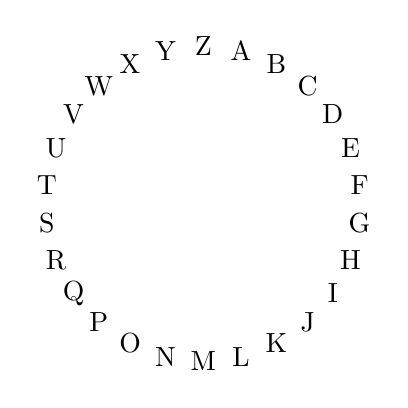
\begin{tikzpicture}
  ...
  \foreach[count=\x] \c in {A, ..., Z} {
    \node at ($(2,2) + (90 - \x * 360/26:2)$) {\c};
  }
  ...
\end{tikzpicture}
\end{lstlisting}
\end{minipage}
\hfill
\begin{minipage}[c]{0.29\textwidth}
  \centering
  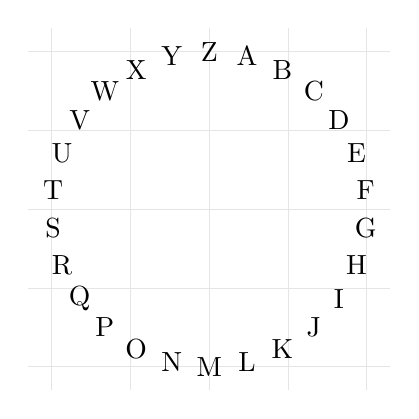
\begin{tikzpicture}
    \draw[gray!20] (-0.3,-0.3) grid (4.3,4.3);
    \foreach[count=\x] \c in {A, ..., Z} {
      \node at ($(2,2) + (90 - \x * 360/26:2)$) {\c};
    }
  \end{tikzpicture}
\end{minipage}

\subsubsection*{Specifying Automatic Ranges}

\begin{minipage}[c]{0.7\textwidth}
\begin{lstlisting}
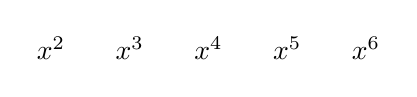
\begin{tikzpicture}
  ...
  \foreach[count=\x from 0] \c in {x^2, x^..., x^6} {
    \node at (\x, 2) {$\c$};
  }
  ...
\end{tikzpicture}
\end{lstlisting}
\end{minipage}
\hfill
\begin{minipage}[c]{0.29\textwidth}
  \centering
  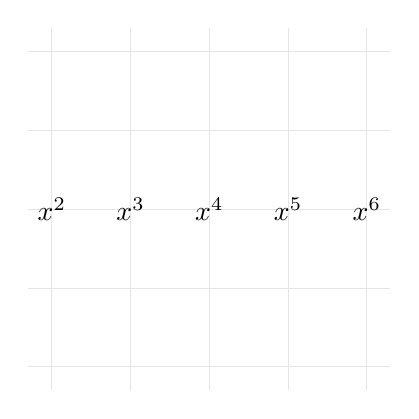
\begin{tikzpicture}
    \draw[gray!20] (-0.3,-0.3) grid (4.3,4.3);
    \foreach[count=\x from 0] \c in {x^2, x^..., x^6} {
      \node at (\x, 2) {$\c$};
    }
  \end{tikzpicture}
\end{minipage}

\subsubsection*{Unpacking variables}
\begin{minipage}[c]{0.7\textwidth}
\begin{lstlisting}
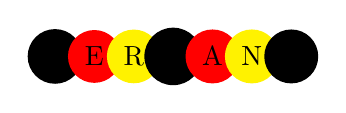
\begin{tikzpicture}
  ...
  \foreach[count=\i from 0] \ch/\col in
  {G/black, E/red, R/yellow, M/black, A/red, N/yellow, Y/black}
  {
    \node[circle, fill=\col] at ({\i/2 + 0.5} , 2) {\ch};
  }
  ...
\end{tikzpicture}
\end{lstlisting}
\end{minipage}
\hfill
\begin{minipage}[c]{0.29\textwidth}
  \centering
  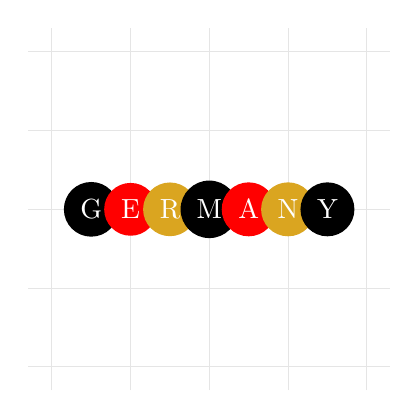
\begin{tikzpicture}
    \draw[gray!20] (-0.3,-0.3) grid (4.3,4.3);
    \foreach[count=\i from 0] \ch/\col in {G/black, E/red, R/Goldenrod, M/black, A/red, N/Goldenrod, Y/black} {
      \node[circle, fill=\col, text=white] at ({\i/2 + 0.5} , 2) {\ch};
    }
  \end{tikzpicture}
\end{minipage}

\section{Plotten}

\section{Arrows}
\subsubsection*{Most common arrow types}

\begin{minipage}[c]{0.7\textwidth}
\begin{lstlisting}
\usetikzlibrary{arrows.meta} % Import necessary

\begin{tikzpicture}
  ...
  \draw[{to}-{To}]             (0,4.0)  -- (4,4.0);
  \draw[{latex}-{Latex}]       (0,3.5)  -- (4,3.5);
  \draw[{stealth}-{Stealth}]   (0,3.0)  -- (4,3.0);
  \draw[{Triangle}-{Triangle}] (0,2.5)  -- (4,2.5);
  \draw[{Diamond}-{Diamond}]   (0,2.0)  -- (4,2.0);
  \draw[{Circle}-{Circle}]     (0,1.5)  -- (4,1.5);
  \draw[{Bar}-{Bar}]           (0,1.0)  -- (4,1.0);
  \draw[{Hooks}-{Hooks}]       (0,0.5)  -- (4,0.5);
  \draw[{Bracket}-{Bracket}]   (0,0.0)  -- (4,0.0);
  ...
\end{tikzpicture}
\end{lstlisting}
\end{minipage}
\hfill
\begin{minipage}[c]{0.29\textwidth}
  \centering
  \begin{tikzpicture}
    \draw[gray!20] (-0.3,-0.3) grid (4.3,4.3);

    \draw[{to}-{To}, thick]           (0,4.0)  -- (4,4.0);
    \draw[{latex}-{Latex}, thick]     (0,3.5)  -- (4,3.5);
    \draw[{stealth}-{Stealth}, thick] (0,3.0)  -- (4,3.0);
    \draw[{Triangle}-{Triangle}, thick] (0,2.5) -- (4,2.5);
    \draw[{Diamond}-{Diamond}, thick] (0,2.0)  -- (4,2.0);
    \draw[{Circle}-{Circle}, thick]   (0,1.5)  -- (4,1.5);
    \draw[{Bar}-{Bar}, thick]         (0,1.0)  -- (4,1.0);
    \draw[{Hooks}-{Hooks}, thick]     (0,0.5)  -- (4,0.5);
    \draw[{Bracket}-{Bracket}, thick] (0,0.0)  -- (4,0.0);

  \end{tikzpicture}
\end{minipage}

\subsubsection*{Shorthands}

\begin{minipage}[c]{0.7\textwidth}
\begin{lstlisting}
\usetikzlibrary{arrows} % Import necessary

\begin{tikzpicture}
  ...
    \draw[<->] (0,3.5) -- (4,3.5);
    \draw[|-|] (0,2.5) -- (4,2.5);
    \draw[o-o] (0,1.5) -- (4,1.5);
    \draw[*-*] (0,0.5) -- (4,0.5);
  ...
\end{tikzpicture}
\end{lstlisting}
\end{minipage}
\hfill
\begin{minipage}[c]{0.29\textwidth}
  \centering
  \begin{tikzpicture}
    \draw[gray!20] (-0.3,-0.3) grid (4.3,4.3);

    \draw[<->,   thick] (0,3.5) -- (4,3.5);
    \draw[|-|,  thick] (0,2.5) -- (4,2.5);
    \draw[o-o,  thick] (0,1.5) -- (4,1.5);
    \draw[*-*,  thick] (0,0.5) -- (4,0.5);

  \end{tikzpicture}
\end{minipage}

\subsubsection*{Colors}

\begin{minipage}[c]{0.7\textwidth}
\begin{lstlisting}
\begin{tikzpicture}
  ...
  \draw[{*[color=blue]}-{*[color=Green]}]
    (0,4) -- (4,4);
  \draw[{*[color=blue, fill=Green]}-{*[color=Green, fill=blue]}]
    (0,2) -- (4,2);
  ...
\end{tikzpicture}
\end{lstlisting}
\end{minipage}
\hfill
\begin{minipage}[c]{0.29\textwidth}
  \centering
  \begin{tikzpicture}[spy using outlines={circle, magnification=2, size=2cm, connect spies}]
    \draw[gray!20] (-0.3,-0.3) grid (4.3,4.3);

    \draw[{*[color=blue]}-{*[color=Green]}, thick] (0,4) -- (4,4);
    \spy[red, size=20pt] on (0.1,4) in node at (0.1,2.75);
    \spy[red, size=20pt] on (3.9,4) in node at (3.9,2.75);

    \draw[{*[color=blue, fill=Green]}-{*[color=Green, fill=blue]}, thick] (0,0) -- (4,0);
    \spy[red, size=20pt] on (0.1,0) in node at (0.1,1.25);
    \spy[red, size=20pt] on (3.9,0) in node at (3.9,1.25);
  \end{tikzpicture}
\end{minipage}

\subsubsection*{Shortcut for custom arrows}

\begin{minipage}[c]{0.7\textwidth}
\begin{lstlisting}
\begin{tikzpicture}
  ...
  \draw[{*[color=blue]}-{*[color=Green]}]
    (0,4) -- (4,4);
  \draw[{*[color=blue, fill=Green]}-{*[color=Green, fill=blue]}]
    (0,2) -- (4,2);
  ...
\end{tikzpicture}
\end{lstlisting}
\end{minipage}
\hfill
\begin{minipage}[c]{0.29\textwidth}
  \centering
  \begin{tikzpicture}[>={Latex[red, length=5mm, width=7mm]}]
    \draw[gray!20] (-0.3,-0.3) grid (4.3,4.3);
    \draw[<->, thick] (0,0) -- (4,4);
  \end{tikzpicture}
\end{minipage}

\newpage
\section{Positioning (a full on example)}

In research papers, especially related to computer science, you often see diagrams as such
\begin{center}

  \begin{tikzpicture}[
      % Styles
      MATMUL/.style={rectangle, draw=black, fill=Plum!30, very thick, minimum size=7mm, rounded corners},
      SOFTMAX/.style={rectangle, draw=black, fill=Green!20, very thick, minimum size=7mm, rounded corners},
      MASK/.style={rectangle, draw=black, fill=red!20, very thick, minimum size=7mm, rounded corners},
      SCALE/.style={rectangle, draw=black, fill=yellow!30, very thick, minimum size=7mm, rounded corners},
    ]
    % Help Grid
    % \draw[gray!20] (-5,-5) grid (15, 15);
    % \foreach \x in {0,...,10} \fill[blue!20] (\x,0) circle (1pt) node[below] {(\x,0)};
    % \foreach \y in {0,...,10} \fill[blue!20] (0,\y) circle (1pt) node[left] {(0,\y)};

    % Nodes
    \node (Q) {Q};
    \node (K) [right=0.25cm of Q] {K};
    \node (V) [right=0.25cm of K] {V};
    \node[MATMUL] (MatMulFirst) at ($(Q)!0.5!(K) + (0,1cm)$) {MatMul};
    \node[SCALE] (Scale) [above=0.5cm of MatMulFirst] {Scale};
    \node[MASK] (Mask) [above=0.5cm of Scale] {Mask (opt.)};
    \node[SOFTMAX] (Softmax) [above=0.5cm of Mask] {Softmax};
    \node[MATMUL] (MatMulSecond) at ($(K)!0.6!(V) + (0,6cm)$) {MatMul};

    % Connections
    \draw[-{Latex}] (Q.north) -- ($(MatMulFirst.south) + (-0.385cm, 0)$);
    \draw[-{Latex}] (K.north) -- ($(MatMulFirst.south) + (0.385cm, 0)$);
    \draw[-{Latex}] (MatMulFirst.north) -- (Scale.south);
    \draw[-{Latex}] (Scale.north) -- (Mask.south);
    \draw[-{Latex}] (Mask.north) -- (Softmax.south);
    \draw[-{Latex}] (V.north) -| ($(MatMulSecond.south) + (0.3126cm, 0)$);
    \draw[-{Latex}, rounded corners] (Softmax.north) -- ++(0,0.25cm) -| ($(MatMulSecond.south) + (-0.385cm, 0)$);
    \draw[-{Latex}] (MatMulSecond.north) -- ($(MatMulSecond) + (0,0.8cm)$);
  \end{tikzpicture}
\end{center}
This requires placing nodes relative to another and is usually done as follows:
\subsubsection*{Defining node styles}
First some styles are defined that can be reused for multiple nodes
\begin{lstlisting}
...
\begin{tikzpicture}[
  % Styles
  MATMUL/.style   = {rectangle, draw=black, fill=Plum!30,   very thick, rounded corners},
  SOFTMAX/.style  = {rectangle, draw=black, fill=Green!20,  very thick, rounded corners},
  MASK/.style     = {rectangle, draw=black, fill=red!20,    very thick, rounded corners},
  SCALE/.style    = {rectangle, draw=black, fill=yellow!30, very thick, rounded corners},
  ]
\end{tikzpicture}
...
\end{lstlisting}
\subsubsection*{Positioning nodes}
You then go on positioning nodes relative to other nodes
\\[4pt]
\begin{minipage}[c]{0.8\textwidth}
\begin{lstlisting}
\begin{tikzpicture}
  [
  % Styles
  ...
  ]
  % Nodes
  \node (Q) {Q};
  \node (K) [right=of Q] {K};
  \node (V) [right=of K] {V};
  \node[MATMUL] (MatMulFirst) at ($(Q)!0.5!(K) + (0,1cm)$) {MatMul};
  \node[SCALE] (Scale) [above=0.5cm of MatMulFirst] {Scale};
  \node[MASK] (Mask) [above=0.5cm of Scale] {Mask (opt.)};
  \node[SOFTMAX] (Softmax) [above=0.5cm of Mask] {Softmax};
  \node[MATMUL] (MatMulSecond) at ($(K)!0.6!(V) + (0,6cm)$) {MatMul};
  ...
\end{tikzpicture}
\end{lstlisting}
\end{minipage}
\hfill
\begin{minipage}[c]{0.19\textwidth}
  \centering
  \begin{tikzpicture}[
      % Styles
      MATMUL/.style={rectangle, draw=black, fill=Plum!30, very thick, minimum size=7mm, rounded corners},
      SOFTMAX/.style={rectangle, draw=black, fill=Green!20, very thick, minimum size=7mm, rounded corners},
      MASK/.style={rectangle, draw=black, fill=red!20, very thick, minimum size=7mm, rounded corners},
      SCALE/.style={rectangle, draw=black, fill=yellow!30, very thick, minimum size=7mm, rounded corners},
    ]

    % Nodes
    \node (Q) {Q};
    \node (K) [right=0.25cm of Q] {K};
    \node (V) [right=0.25cm of K] {V};
    \node[MATMUL] (MatMulFirst) at ($(Q)!0.5!(K) + (0,1cm)$) {MatMul};
    \node[SCALE] (Scale) [above=0.5cm of MatMulFirst] {Scale};
    \node[MASK] (Mask) [above=0.5cm of Scale] {Mask (opt.)};
    \node[SOFTMAX] (Softmax) [above=0.5cm of Mask] {Softmax};
    \node[MATMUL] (MatMulSecond) at ($(K)!0.6!(V) + (0,6cm)$) {MatMul};
  \end{tikzpicture}
\end{minipage}

\newpage
\subsubsection*{Connecting nodes}
Lastly you connect the nodes
\\[4pt]
\begin{minipage}[c]{0.8\textwidth}
\begin{lstlisting}
\begin{tikzpicture}
  [
  % Styles
  ...
  ]
  % Nodes
  ...
  % Connections
  \draw[-{Latex}] (Q.north) -- ($(MatMulFirst.south) + (-0.385cm, 0)$);
  \draw[-{Latex}] (K.north) -- ($(MatMulFirst.south) + (0.385cm, 0)$);
  \draw[-{Latex}] (MatMulFirst.north) -- (Scale.south);
  \draw[-{Latex}] (Scale.north) -- (Mask.south);
  \draw[-{Latex}] (Mask.north) -- (Softmax.south);
  \draw[-{Latex}] (V.north) -| ($(MatMulSecond.south) + (0.3126cm, 0)$);
  \draw[-{Latex}, rounded corners] (Softmax.north) -- ++(0,0.25cm) -| ($(MatMulSecond.south) + (-0.385cm, 0)$);
  \draw[-{Latex}] (MatMulSecond.north) -- ($(MatMulSecond) + (0,0.8cm)$);
  ...
\end{tikzpicture}
\end{lstlisting}
\end{minipage}
\hfill
\begin{minipage}[c]{0.19\textwidth}
  \centering
 \begin{tikzpicture}[
      % Styles
      MATMUL/.style={rectangle, draw=black, fill=Plum!30, very thick, minimum size=7mm, rounded corners},
      SOFTMAX/.style={rectangle, draw=black, fill=Green!20, very thick, minimum size=7mm, rounded corners},
      MASK/.style={rectangle, draw=black, fill=red!20, very thick, minimum size=7mm, rounded corners},
      SCALE/.style={rectangle, draw=black, fill=yellow!30, very thick, minimum size=7mm, rounded corners},
    ]
    % Help Grid
    % \draw[gray!20] (-5,-5) grid (15, 15);
    % \foreach \x in {0,...,10} \fill[blue!20] (\x,0) circle (1pt) node[below] {(\x,0)};
    % \foreach \y in {0,...,10} \fill[blue!20] (0,\y) circle (1pt) node[left] {(0,\y)};

    % Nodes
    \node (Q) {Q};
    \node (K) [right=0.25cm of Q] {K};
    \node (V) [right=0.25cm of K] {V};
    \node[MATMUL] (MatMulFirst) at ($(Q)!0.5!(K) + (0,1cm)$) {MatMul};
    \node[SCALE] (Scale) [above=0.5cm of MatMulFirst] {Scale};
    \node[MASK] (Mask) [above=0.5cm of Scale] {Mask (opt.)};
    \node[SOFTMAX] (Softmax) [above=0.5cm of Mask] {Softmax};
    \node[MATMUL] (MatMulSecond) at ($(K)!0.6!(V) + (0,6cm)$) {MatMul};

    % Connections
    \draw[-{Latex}] (Q.north) -- ($(MatMulFirst.south) + (-0.385cm, 0)$);
    \draw[-{Latex}] (K.north) -- ($(MatMulFirst.south) + (0.385cm, 0)$);
    \draw[-{Latex}] (MatMulFirst.north) -- (Scale.south);
    \draw[-{Latex}] (Scale.north) -- (Mask.south);
    \draw[-{Latex}] (Mask.north) -- (Softmax.south);
    \draw[-{Latex}] (V.north) -| ($(MatMulSecond.south) + (0.3126cm, 0)$);
    \draw[-{Latex}, rounded corners] (Softmax.north) -- ++(0,0.25cm) -| ($(MatMulSecond.south) + (-0.385cm, 0)$);
    \draw[-{Latex}] (MatMulSecond.north) -- ($(MatMulSecond) + (0,0.8cm)$);
  \end{tikzpicture}
\end{minipage}

\end{document}
